\documentclass[12pt]{extarticle}
\usepackage{preamble}
\geometry{letterpaper, landscape, margin=0.5in}
\renewcommand{\answer}[1]{}
\setlength{\parskip}{4pt}

\begin{document}
\pagestyle{empty}

\daybanner{Unit 1 \textperiodcentered\ Topics 1.4--1.8 (CED 1.4--1.8) \textperiodcentered\ THE PROBLEM}{Candle Tests: Choosing the Evidence}

\noindent\begin{minipage}[t]{0.57\linewidth}
\vspace{0pt}
Suppose a candle workshop tests 12 candles. It records wax type and burn duration in hours. A and B summarize wax type for these same 12 candles; C and D summarize their burn durations. The links between wax type and duration are not shown. Histogram bins include the left endpoint and exclude the right endpoint; each dot represents one candle.\par\smallskip
The report must identify the most common wax type and the number of candles that burned exactly 5 hours. An editor proposes: \emph{Keep only B and C. B changes which wax is most common because its bars are taller than A's. C shows five candles at exactly 5 hours, so D adds nothing needed.}\par
\end{minipage}\hfill
\begin{minipage}[t]{0.40\linewidth}
\vspace{0pt}
\begin{center}
\begin{tabular}{cc}
\begin{tikzpicture}\begin{axis}[width=0.43\linewidth,height=1.38in,ybar,ymin=0,ymax=7,ytick={0,2,4,6},symbolic x coords={Beeswax,Soy,Paraffin},xtick=data,bar width=14pt,ylabel={Candles},title={A: Wax counts},tick label style={font=\scriptsize},label style={font=\scriptsize},title style={font=\small},nodes near coords]
\addplot[fill=calloutblue] coordinates {(Beeswax,6) (Soy,4) (Paraffin,2)};
\end{axis}\end{tikzpicture}&
\begin{tikzpicture}\begin{axis}[width=0.43\linewidth,height=1.38in,ybar,ymin=0,ymax=60,ytick={0,20,40,60},symbolic x coords={Beeswax,Soy,Paraffin},xtick=data,bar width=14pt,ylabel={Percent},title={B: Wax percents},tick label style={font=\scriptsize},label style={font=\scriptsize},title style={font=\small}]
\addplot[fill=calloutblue] coordinates {(Beeswax,50) (Soy,33.3333) (Paraffin,16.6667)};
\node[font=\scriptsize,anchor=south] at (axis cs:Beeswax,50) {50};
\node[font=\scriptsize,anchor=south] at (axis cs:Soy,33.3333) {$33\frac13$};
\node[font=\scriptsize,anchor=south] at (axis cs:Paraffin,16.6667) {$16\frac23$};
\end{axis}\end{tikzpicture}\\
\begin{tikzpicture}\begin{axis}[width=0.43\linewidth,height=1.38in,ybar interval,x tick label as interval=false,bar shift=0pt,xmin=0,xmax=12,ymin=0,ymax=7,xtick={0,4,8,12},ytick={0,1,2,3,4,5,6},xlabel={Burn duration (hours)},ylabel={Candles},title={C: Duration histogram},tick label style={font=\scriptsize},label style={font=\scriptsize},title style={font=\small}]
\addplot[fill=calloutblue] coordinates {(0,6) (4,5) (8,1) (12,0)};
\end{axis}\end{tikzpicture}&
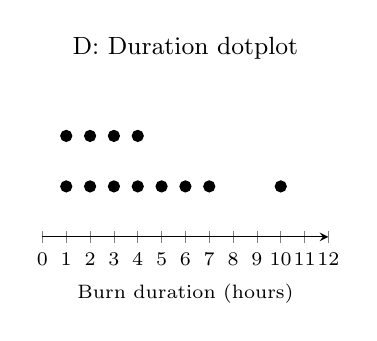
\begin{tikzpicture}\begin{axis}[width=0.43\linewidth,height=1.38in,xmin=0,xmax=12,ymin=0,ymax=3,xtick={0,1,...,12},ytick=\empty,axis y line=none,axis x line=bottom,xlabel={Burn duration (hours)},title={D: Duration dotplot},tick label style={font=\scriptsize},label style={font=\scriptsize},title style={font=\small}]
\addplot[only marks,mark=*,mark size=2pt] coordinates {(1,1) (1,2) (2,1) (2,2) (3,1) (3,2) (4,1) (4,2) (5,1) (6,1) (7,1) (10,1)};
\end{axis}\end{tikzpicture}
\end{tabular}
\end{center}
\end{minipage}

\begin{firsttakebox}{FIRST TAKE --- one sentence before you work the parts}
Which part of the proposed report needs the closest check, and why?
\end{firsttakebox}

\begin{description}[leftmargin=1.15in, labelwidth=1in, itemsep=2pt, topsep=2pt]
  \item[\dokbadge{1}~(a)] Name the categorical variable in A and give one of its categories. Name the quantitative variable in C and its unit.
  \item[\dokbadge{2}~(b)] Convert each count in A to a percent and compare with B. Explain whether these graphs represent different category distributions. \textbf{Check your response:} \fbox{\rule{0pt}{0.65em}\hspace{0.65em}} all three categories; \fbox{\rule{0pt}{0.65em}\hspace{0.65em}} total used; \fbox{\rule{0pt}{0.65em}\hspace{0.65em}} axis units.
  \item[\dokbadge{2}~(c)] Compare what the bar from 4 to 8 in C tells you with the dots over that interval in D. State the interval count and every individual duration there, including repeats. Explain the difference in precision, using candles and hours.
  \item[\dokbadge{3}~(d)] $\star$ Evaluate the editor\textquotesingle s plan in a short paragraph. Defend a set of displays sufficient for both reporting questions and correct any unsupported claims using numerical evidence. The teacher scores this response E/P/I by hand; nothing is automatically scored.
\end{description}

\vfill
\textbf{Self-paced bonus problem. Work (a)--(d) from this sheet; turn it in whenever you finish.}

\end{document}
